\chapter{Conclusions}

The knowledge on elementary particles collected along decades of experimental searches accompanied by theoretical and technological developments, established the standard model as the most suitable theory to describe three fundamental forces: strong, weak, and electromagnetic. The gravitational force also plays an important role in the description of the universe, however, its connection with the other fundamental forces is still not well understood.

It is possible to overcome the difficulties of a common description of gravity and the standard model via unification approach, as long as the predictions of the new theory be susceptible of experimental demonstration. In this thesis, special attention is paid to a model that not only predicts the existence of a previously unobserved particle, but also establishes the existence of extra dimensions. In fact, the bulk graviton arises in the context of warped extra dimensional models, and its existence can be revealed through the analysis of data collected by the CMS experiment. 

Our search targets a heavy resonance at the TeV scale producing two leptons and one jet in the final state, coming from the intermediate decay of two vector bosons. Similar searches were performed by CMS using proton-proton collision data collected in 2012 at center-of-mass energy $\sqrt{s} = 8$ TeV, and more recently, using 2016 data at $\sqrt{s}=13$ TeV. 

This thesis presents the analysis of the CMS 2015 data corresponding to an integrated luminosity of 2.7 fb$^{-1}$ collected at $\sqrt{s}=13$ TeV. Our results \cite{CMS-PAS-B2G-16-010} are compatible with previous \cite{Khachatryan:2014gha} and posterior \cite{CMS-PAS-B2G-16-022,CMS-PAS-HIG-16-034} searches in the mass range 0.8 - 2.5 TeV, showing no excess above the standard model prediction. Given the reduced statistics in data and the low cross section of the benchmark model (bulk graviton with $k/M_{Pl}=0.5$), our analysis did not reach the sensitivity required to establish exclusion limits on the theoretical cross section of the model under study.

\section*{Outlook of the LHC}
While no new physics has yet been seen at the LHC, many models have been eliminated or have had their parameter space quite limited. The experimental approach to the searches is independent of the details of the specific production or decay patterns, and the sensitivity for observing new physics signals largely depends on the available luminosity. 

There are plans to increase the luminosity of the LHC above the original design, extending the physics program for the high luminosity LHC \cite{Contardo:2020886}. The second phase of the LHC will provide an additional integrated luminosity of about 2,500 fb$^{-1}$ over 20 years of operation (Fig. \ref{hllhc}), enlarging the discovery potential of new particles.

\begin{figure}[ht]
\centering
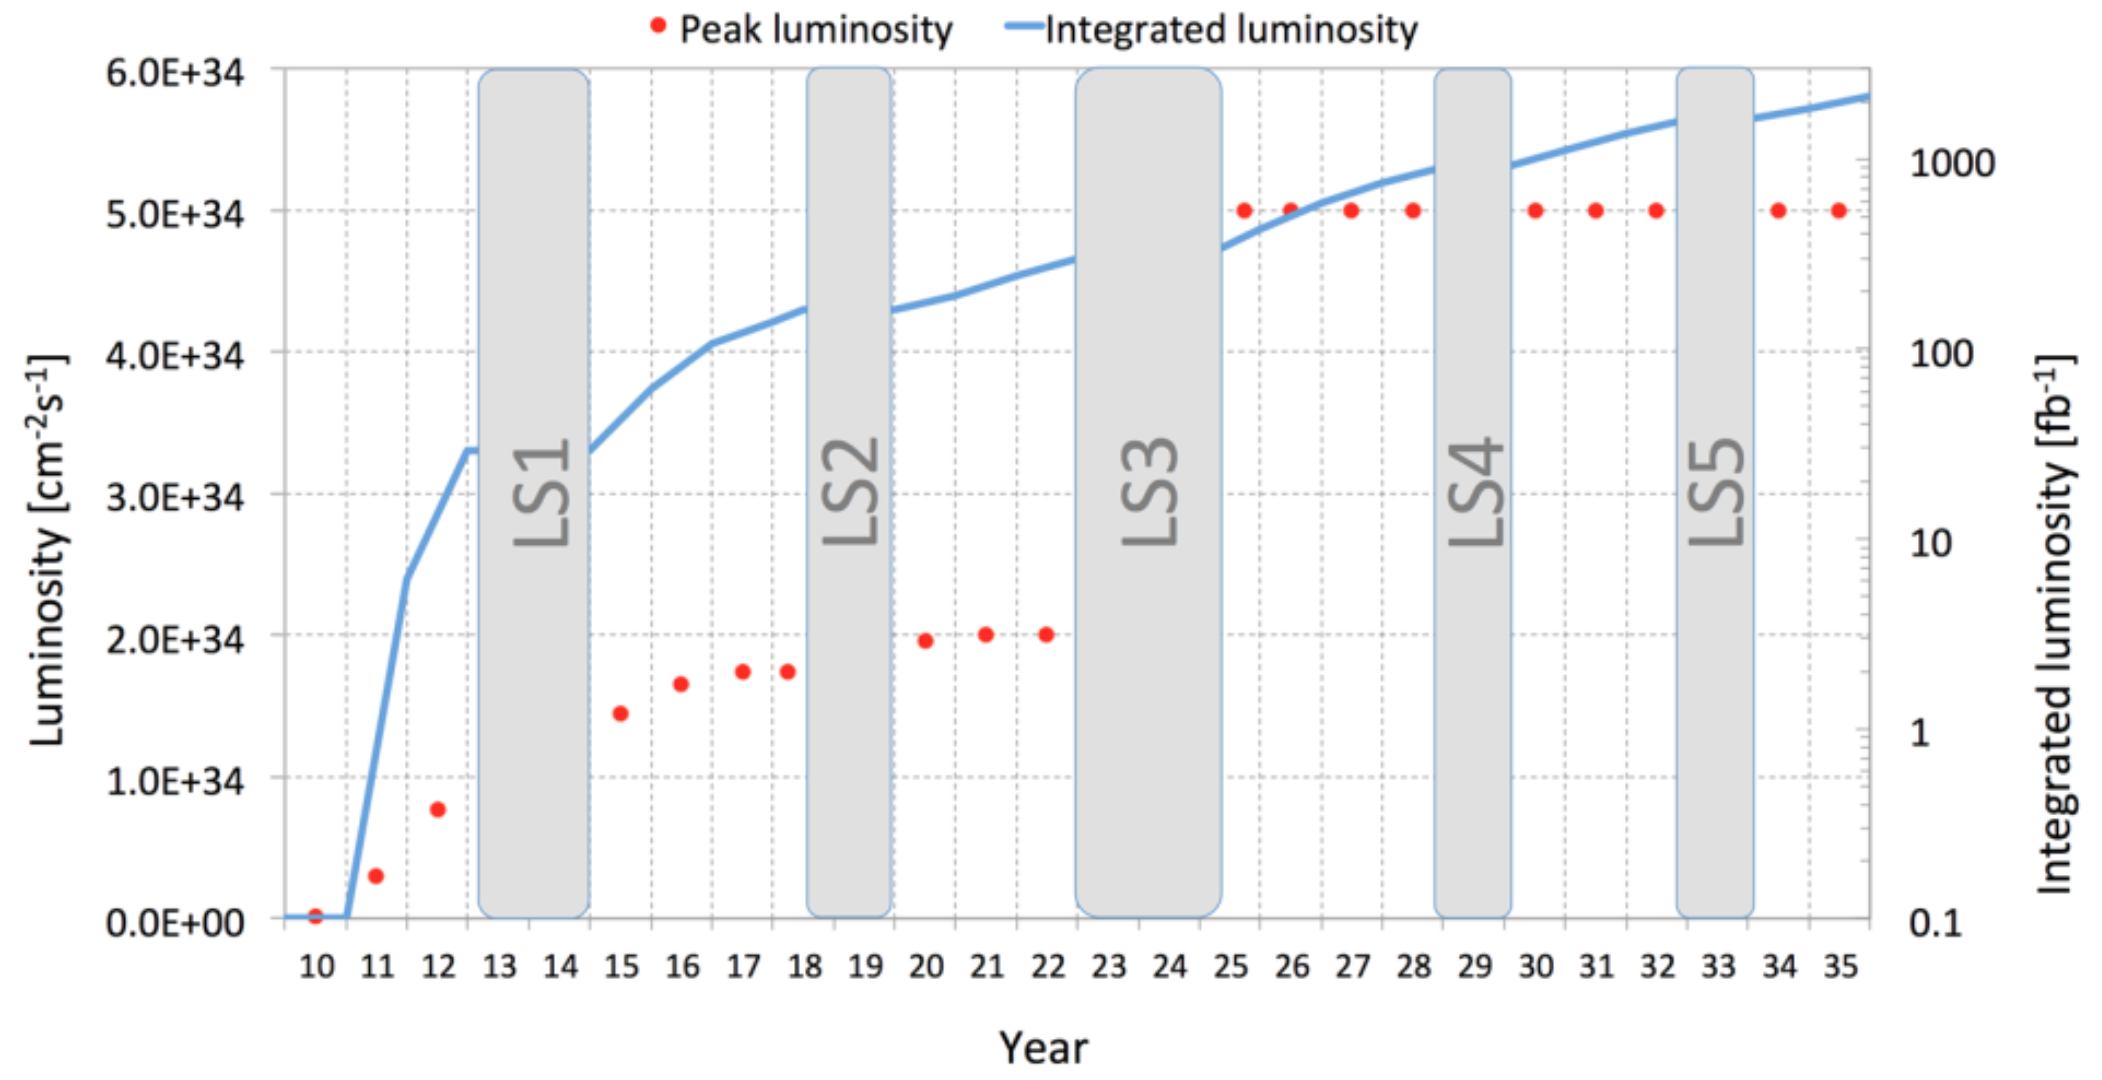
\includegraphics[scale=0.40]{figures/experiment/hllhc.png} 
\caption[Luminosity plans of the HL-LHC]{Projected LHC performance through 2035, showing preliminary dates for long shutdowns \cite{Contardo:2020886}.}
\label{hllhc}
\end{figure}

